\RequirePackage{fix-cm}

\documentclass[twocolumn,draft,natbib]{svjour3}
\smartqed  % flush right qed marks, e.g. at end of proof

\usepackage{graphicx}

% Tables
\usepackage{multirow}
\usepackage{colortbl}
\usepackage{booktabs}
\usepackage[algoruled,vlined]{algorithm2e}


\journalname{Autonmous Robots}
\begin{document}

%%%%%%%%%%%%%%%%%%%%%%%%%%%%%%%%%%%%%%%%%%%%%%%%%%%%%%%%%%%%%%%%%%%%%%%%%%%%%%%%
\title{GPAtlasRRT: A probabilistic next-best tactile action strategy for object shape modelling and exploration
  \thanks{This work is supported by EC-FP7-ICT-600918, PacMan.}
}
%\subtitle{GPAtlasRRT: Gaussian Process for shape modelling, continuation method on implicit manifolds (Atlas), rapidly-exploring random trees}
%\titlerunning{Short form of title}

\author{Carlos J. Rosales         \and
        Claudio Zito              \and
        Federico Spinelli         \and \\
        Jeremy L. Wyatt           \and
        Marco Gabiccini           \and
}

\institute{C. J. Rosales, F. Spinelli, and M. Gabiccini \at
              Centro di Ricerca ``E. Piaggio'', Univ. di Pisa, Italy. \\
              Tel.: +39 (050) 2217050\\
              \email{carlos.rosales@for.unipi.it}           %
           \and
           C. Zito and J. L. Wyatt \at
              Intelligent Robotics Laboratory, Univ. of Birmingham, UK.\\
              Tel.: +44 (0) 121 415 8722\\
              \email{cxz004@cs.bham.ac.uk}              %
}

\date{Received: date / Accepted: date}
% The correct dates will be entered by the editor


\maketitle

%%%%%%%%%%%%%%%%%%%%%%%%%%%%%%%%%%%%%%%%%%%%%%%%%%%%%%%%%%%%%%%%%%%%%%%%%%%%%%%%
\begin{abstract}
Gaussian Process are state-of-the-art techniques for regression, and recently been used for shape representation. They have been recently used to model manifolds and implicitly defined surfaces. The second using thin-plate interpolation and variational concepts.
%Moreover, shape matching methods are useful for object recognition.
Continuation methods are used in many ways, typically to find local parametrizations of implicitly defined manifolds. Each parametrization is called a chart, and it should provide a one-to-one map from the parametric space onto the manifold, that is, it should cover an area over the manifold. The manifold is then globally parametrized or fully covered by a collection of charts properly coordinated to not overlap the covered regions called an atlas. The names suggest already the navigation purpose.
Rapidly-exploring random trees are a probabilistic framework to explore complex search spaces. The idea is to grow trees at random or biased directions to ``evenly'' the space from a root node. However, using several root nodes is also possible.
The two latter has been succesfully combined to explore the interesting regions of the manifold for the problem at hand, introduced as AtlasRRT.
This is a well-suited framework for object shape modelling and exploraion via tactile actions, as we propose the GPAtlasRRT strategy for that. The basic idea is to use Gaussian Process implicit surfaces for the shape representation, and then explore the relevant regions of the shape that will improve the model via continuation methods and rapidly-epxloring random tree techniques.
\keywords{Active exploration \and
          Next-best tactile exploration action \and
          Object shape modelling}
\end{abstract}

%%%%%%%%%%%%%%%%%%%%%%%%%%%%%%%%%%%%%%%%%%%%%%%%%%%%%%%%%%%%%%%%%%%%%%%%%%%%%%%%
\section{Introduction}
\label{sec:intro}


%%%%%%%%%%%%%%%%%%%%%%%%%%%%%%%%%%%%%%%%%%%%%%%%%%%%%%%%%%%%%%%%%%%%%%%%%%%%%%%%
%\section{Related work}
%\label{sec:soa}

General guidelines : \citet{Bajcsy1989Machine}

Vision-based exploration is the most studied, perhaps due to its non-invasive nature, which avoids the contact between rigid bodies which is the cause of most headaches in physics modelling, simulation and control.

As very well said by \citet{Petrovskaya2011Global}, even when initial works date back to the 80's, tactile perception has not been addressed as deeply as the non-invasive counterpart, visual perception. Besides the need of being actively controlled, tactile sensors typically required ad-hoc mechanical devices.

``Touch-based perception has not been studied in as much depth
as vision because standardized touch sensors are not as easily
available. In many situations, tactile sensors have to be hand
crafted specifically for the robot and the task. This complicates
comparisons between methods and slows progress in tactile
perception. However, recently there has been a surge of interest
in the field due to the necessity of touch-based perception in
service applications''

Whereas \citet{Petrovskaya2011Global} is more interested in the object pose estimation problem, here we are more interested in the object shape modelling, sort of in the mapping of rather than localization in a SLAM problem.

On active touch sensing \citet{Prescott2011Active}

% There are two broad directions to represent object shapes. Use either an implicit or an explicit (a.k.a. parametric) representation. A good comparison between the two is provided by \citet{Pirri2006About}.

Regarding the shape representation...

Using Gaussian Process for shape modelling is having an intensive development in recent years \citep{Mahler2015Grasp,Rosales2014Active,Bjorkman2013Enhancing,Dragiev2011Gaussian}, due to its versatility to accomadate noisy information, provide smooth regression of data, and a natural way to fuse different sources of information \citep{Rasmussen2006Gaussian}.

Manifold gaussian process: \citet{Calandra2014Manifold} ``The quality of a Gaussian Process model strongly depends on an appropriate covariance function.''

The tree is constructed incrementally from samples drawn randomly from the search space and is inherently biased to grow towards large unsearched areas of the problem
Space-filling trees are 
Rapidly-exploring random trees \citet{LaValle2011Motion}

Continuation method for implicitly defined surfaces \citet{Henderson1993COMPUTING}

More general continuation method used in a more complex scenario combined with rapidly-exploring random trees \citep{LaValle2011Motion} by \citet{Jaillet2013Path}, where the idea is to explore the part of the manifold defined by several kinematic loop constraints that solves the motion planning query.

\citet{Zhu2009Nonrigid} succesfully recover non-rigid shape, means that gaussian processes can be used

\citet{Dragiev2011Gaussian} uses a squared-exponential-like covariance function. This is selection seems to be in agreement with the use is given to the shape estimation as a gradient field that drives the reach-to-grasp controller in a smooth way.

\citet{Rosales2014Active} exploits the Gaussian Process modelling the object shape to find geodesic trajectories on the surface that are later followed by an exploratory probe to gather frictional properties. However, no further use of that propery is given.

\citet{Mahler2015Grasp} proposes similar ideas as those given in \citet{Dragiev2011Gaussian}, in fact they follow the same covariance function for the shape modelling, but adds a local optimization step to have a more elaborated grasp controller that drives the hand to the most-likely succesful object grasp using a metric that involves the well-known Ferrari-Canny measure.

\citet{Williams2007Gaussian} derives the thin-plate covariance function for 3D shapes represented by implicit functions. The property of the thin-plate function to keep the tendency outside the training data is ideal for tactile exploration~\citep[Fig.~2]{Williams2007Gaussian}

The early work by \citet{Allen1987Robotic} presents a hierarchical representation of the object. The tactile exploration strategy to refine is driven by local geometry features. This is engaged by using surface tracing algorithms. In that work, it is literally said: ``Given a starting and ending point on a surface, the sensor traces along the surface reporting its contact positions and normals as it moves along.'' However, no indication is given in how to determine those starting and ending points on the surface.

\citet{Bjorkman2013Enhancing} follows the covariance function derived by \citet{Williams2007Gaussian}. This is the closest work to ours among the references. The main difference being the space in which the best-next exploratory action is computed and the terminal condition for the overal algorithm, and the descriptor. The Zernike moments imply an extra computation time, and lack of a probabilistic interpretation, which it is one of the good things about using Gaussian Process in first place. The exploratory actions are searched in a discrete space in the vertical direction and the approach angle, which seem extrinsic to the shape model. Using this space does not guarantee that the new observations will be on the desired shape region to be explored.  Finally, the number of actions, or touches in this case, are limited to a certain number, and then ordered according to the closes point on the implicit function with higher variance. In contrast, we set the highest expected variance in the shape prediction, so we explore until, probabilistically speaking, that goal is achieved.

% They claim that touch sensing is low bandwith, local, sequential process with better signal-to-noise ratio than vision. 

% Vision is global, has high bandwidth, and is noisy. Touch is a low bandwidth, local, sequential process with better noise properties than vision.

On how to do classification...

Shape representation and descriptor review \citet{Zhang2004Review}

In this work, we provide a systematic and coherent methodology to plan the next-best tactile exploratory action. The tactile exploratory action is intrinsically a contact hypothesis that need to be accepted or discarded after execution. Should the result be any of the two, it helps to improve the object shape prediction up to a pre-specified variability. In contrast to \citet{Bjorkman2013Enhancing}, we propose the same shape representation as descriptor for classification purposes using shape matching techniques~\citep{Belongie2002Shape}. The scope and problem statement is detailed in Sect.~\ref{sec:scope}. The proposed solution is broaden in Sect.~\ref{sec:solution}. The experimental results and discusion is presented in Sect.~\ref{sec:experiments}. Finally, the conclusions and points deserving further attention as given in Sect.~\ref{sec:conclusions}. 
%Reading the paper along watching the attached media is suggested for a better cath-up of the ideas.

%%%%%%%%%%%%%%%%%%%%%%%%%%%%%%%%%%%%%%%%%%%%%%%%%%%%%%%%%%%%%%%%%%%%%%%%%%%%%%%%
\section{Scope}
\label{sec:scope}

We rely on previous works that have proved useful object shape representations via Gaussian Processs in the derivation of grasp controllers.

%%%%%%%%%%%%%%%%%%%%%%%%%%%%%%%%%%%%%%%%
\subsection{Equipment specification}
\label{sec:equipment}

The vision system should be able to provide an initial guess on the object location and observation points on the surface. This is not an strict requirement, since one might be completely blind and still recognize objects around \citep[see e.g.]{Petrovskaya2011Global}. However, the use of an initial set of observation can be done quickly using RGBD sensors to speed up the overall process. 

It is true that mounting the camera as the end-effector of a robot might allow a full object scanning, but there might be cases where this  might not be possible either due to reaching limitations or even sensing capabilities on reduced spaces.

%%%%%%%%%%%%%%%%%%%%%%%%%%%%%%%%%%%%%%%%
\subsection{Assumptions}
\label{sec:limitations}

We assume that a point cloud of a segmented object is provided. However, we provide an optional pre-processing step that shows a reasonably way to do it when the object model is unkown.

Workspace. This is not to be thought as the workspace of a robot, but of the strategy algorithm that works on top of the object shape model. That is, we assume that we are modelling and exploring household objects that can be grasped and manipulated using a human-sized hand. This is specially useful in cases where the predicted shape is not bounded using the given observations, so this workspace will shrink the predicted shape to prevent the robot from going to an empty space, or worst, hitting undesirebly. 

We consider contact to appear when the force torque sensor measures a value higher than $1$N. The robot motion is set slow such that inertial forces are not reflected on the measurements. This is done for safety reasons, since in the phase when the robot is approaching, there is a stop signal if this threshold is superated.

%%%%%%%%%%%%%%%%%%%%%%%%%%%%%%%%%%%%%%%%
\subsection{Problem statement}
\label{sec:problem}

Considering the equipment limitations~\ref{sec:equipment} and the assumptions~\ref{sec:limitations}, the problem for which we propose a solution can be stated as:

Given a point cloud of an object, $\mathcal{O}$, find a suitable represention for the shape that can be exploited for tasks such as object identification and grasping, and a coherent strategy to improve the representation independent of external references, i.e. intrinsic or exploiting the representation, and flexible enough to generate different exploratory actions such as poking points and sliding paths.

%%%%%%%%%%%%%%%%%%%%%%%%%%%%%%%%%%%%%%%%%%%%%%%%%%%%%%%%%%%%%%%%%%%%%%%%%%%%%%%%
\section{Solution}
\label{sec:solution}

First, we provide a pre-processing step with the objective of having a segmented point set of the object \ref{sec:pre}. This is then used to create the probabilistic shape representation \ref{sec:object}. This is then exploited in 

%%%%%%%%%%%%%%%%%%%%%%%%%%%%%%%%%%%%%%%%
\subsection{Pre-processing}
\label{sec:pre}

Given a point cloud of the current scene, say an object on a table, the ubiquituos tabletop object segmentation 
\citep{TabletopObjectDetector} can be used to have 

%%%%%%%%%%%%%%%%%%%%%%%%%%%%%%%%%%%%%%%%
\subsection{Shape modelling}
\label{sec:object}

\begin{algorithm}[h]
\textbf{\textsc{FitGaussianProcess}}$(P, params)$\\ %functionname
\LinesNumbered
\DontPrintSemicolon
\SetAlgoVlined \SetKwInOut{Input}{input} \SetKwInOut{Output}{output}
\Input{The segmented object shape in form of a point cloud, $P$, and the
to be used for the Gaussian Process fitting.}
\Output{The shape model}
  Generate inside and outside points \\
  Merge and label data into the training data $X$ \\
  $\mathcal{GP} \leftarrow$ \textsc{InitModel}$(params)$ \\
  $\mathcal{GP} \leftarrow$ \textsc{FitToData}$(X)$ \\
  \Return $\mathcal{GP}$ \\
\caption{The object shape model generation} \label{algo:strategy}
\end{algorithm}

%%%%%%%%%%%%%%%%%%%%%%%%%%%%%%%%%%%%%%%%
\subsection{Explorattion strategy}
\label{sec:strategy}


\begin{algorithm}[h]
\textbf{\textsc{GPAtlasRRT}}$(\mathcal{GP}, V_{max}, type)$\\ %functionname
\LinesNumbered
\DontPrintSemicolon
\SetAlgoVlined \SetKwInOut{Input}{input} \SetKwInOut{Output}{output}
\Input{The GP The action $type$ can have for now two values, $poke$ for a single
touch, $slide$ for path. This depends on the available hardware.}
\Output{The best next point if any, otherwise null.}
  $e \leftarrow 1$ \\
  \While { $e < h$ } 
  {
    $i \leftarrow 0$ \\
    \While{ $i<n$ }
    {
      \Return action 
    }
    $e \leftarrow e + 1$ \\
  }
  \Return{\sc Null}

\caption{The best-next action planner} \label{algo:strategy}
\end{algorithm}

%%%%%%%%%%%%%%%%%%%%%%%%%%%%%%%%%%%%%%%%
\subsection{Solution in a nutshell}
\label{sec:summary}

\begin{algorithm}[h]
\textbf{\textsc{ObjectShapeExploration}}$(P, V_{max}, type, params)$\\ %functionname
\LinesNumbered
\DontPrintSemicolon
\SetAlgoVlined \SetKwInOut{Input}{input} \SetKwInOut{Output}{output}
\Input{Point cloud of the segmented object}
\Output{The object model predicting the shape up to the specified value $V_{max}$}
  PreProcessing \\
  $\mathcal{GP} \leftarrow $\textsc{FitGaussianProcess}$(P, params)$\\
  \While { \texttt{true} } 
  {
    $a \leftarrow $\textsc{GPAtlasRRT}$(\mathcal{GP}, V_{max}, type)$ \\
    \eIf{ $a$ = \sc Null }
    {
      \Return {$\mathcal{GP}$} \\
    }
    {
      \textsc{ApproachTo}($a$) \\
      \textsc{Execute}($a$) \\
    }
  }
  \Return 

\caption{Best-next action method} \label{algo:strategy}
\end{algorithm}

In the \textsc{ApproachTo} phase, the robot moves using position control and collision avoidance. In the \textsc{Execute} phase, the robot moves using Cartesian impedance control, with the Cartesian force, pose and impedance set properly for the given setup. Implementation details of the solution depicted in Algorithm~\ref{alg:strategy} are given in the next section.


%%%%%%%%%%%%%%%%%%%%%%%%%%%%%%%%%%%%%%%%%%%%%%%%%%%%%%%%%%%%%%%%%%%%%%%%%%%%%%%%
\section{Experiments}
\label{sec:experiments}


\subsection{Apparatus}
\label{sec:apparatus}

We repeat the exploratory probe given in~\citet{Rosales2014Active}. The probe is composed of a semispherical tip (radius $2$cm) on top of an ATI Nano 17 and an in-parallel passive compliant coupler to safely attach it as the end-effector of the 7 degrees of freedom KUKA LWR 4+ robot arm.

The object is grasped by a soft-hand. The 
assumption that the object is unknown holds to the adaptability of the hand.
There is no need to have a precise model of the object, but a rough 
approximation of the shape. The hand softness will do the rest. This setup
complies with the specifications given in Sect.~\ref{sec:equipment}.

\subsection{Results}
\label{sec:results}

%%%%%%%%%%%%%%%%%%%%%%%%%%%%%%%%%%%%%%%%%%%%%%%%%%%%%%%%%%%%%%%%%%%%%%%%%%%%%%%%
\section{Conclusions and future directions}
\label{sec:conclusions}


%%%%%%%%%%%%%%%%%%%%%%%%%%%%%%%%%%%%%%%%%%%%%%%%%%%%%%%%%%%%%%%%%%%%%%%%%%%%%%%%
\begin{acknowledgements}
The authors would like to thank E. Farnioli for the fruitful discussions and 
initial matlab implementations about Gaussian Processes, as well as to G. 
Santaera for the support with the sensorized glove.
\end{acknowledgements}

%%%%%%%%%%%%%%%%%%%%%%%%%%%%%%%%%%%%%%%%%%%%%%%%%%%%%%%%%%%%%%%%%%%%%%%%%%%%%%%%
\bibliographystyle{spbasic}
\bibliography{bib/report}

\end{document}
% end of file

%%%%%%%%%%%%%%%%%%%%%%%%%%%%%%%%%%%%%%%%%%%%%%%%%%%%%%%%%%%%%%%%%%%%%%%%%%%%%%%%
%% HELPS
% \begin{equation}
% a^2+b^2=c^2
% \end{equation}
%
% \begin{figure}
% \centering
%   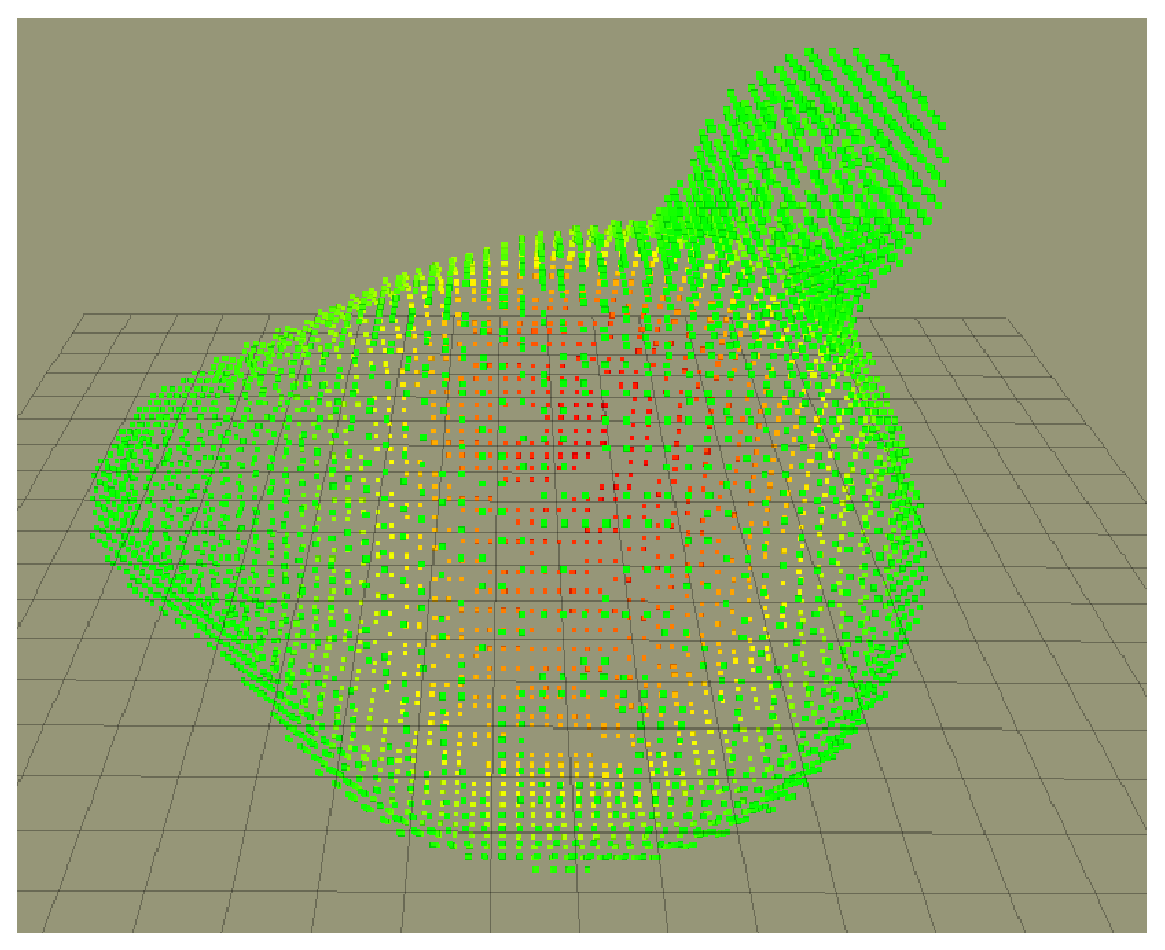
\includegraphics{example.eps}
% \caption{Please write your figure caption here}
% \label{fig:1}
% \end{figure}
%
% \begin{figure*}
% \centering
%   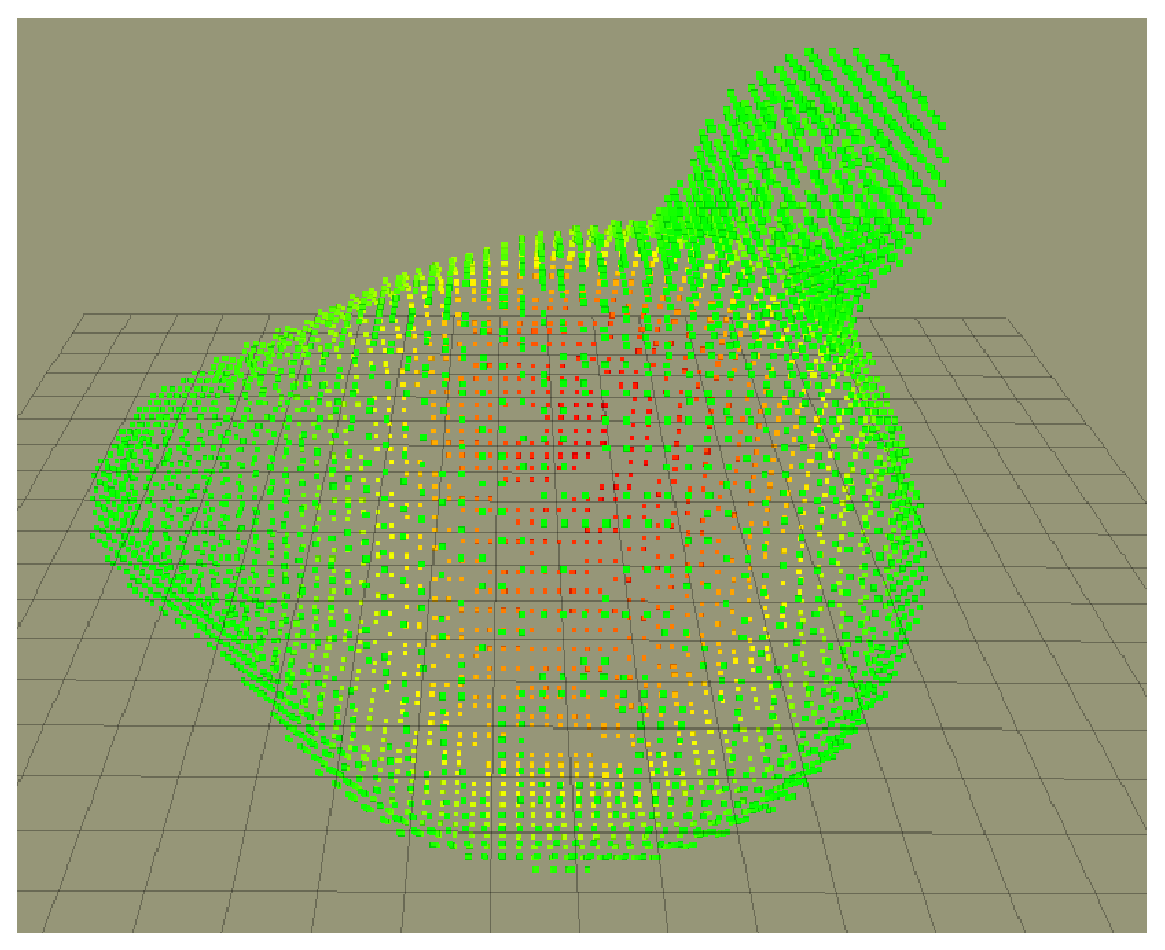
\includegraphics[width=0.75\textwidth]{example.eps}
% \caption{Please write your figure caption here}
% \label{fig:2}
% \end{figure*}
%
% % For tables use
% \begin{table}
% \caption{Please write your table caption here}
% \label{tab:1}
% \begin{tabular}{lll}
% \hline\noalign{\smallskip}
% first & second & third  \\
% \noalign{\smallskip}\hline\noalign{\smallskip}
% number & number & number \\
% number & number & number \\
% \noalign{\smallskip}\hline
% \end{tabular}
% \end{table}
%%%%%%%%%%%%%%%%%%%%%%%%%%%%%%%%%%%%%%%%%%%%%%%%%%%%%%%%%%%%%%%%%%%%%%%%%%%%%%%%